\documentclass{beamer}

\usepackage{graphicx}
\usepackage[latin1]{inputenc}
\usepackage[T1]{fontenc}
\usepackage[english]{babel}
\usepackage{listings}
\usepackage{xcolor}
\usepackage{eso-pic}
\usepackage{mathrsfs}
\usepackage{url}
\usepackage{amssymb}
\usepackage{amsmath}
\usepackage{multirow}
\usepackage{hyperref}
\usepackage{booktabs}
% \usepackage{bbm}
\usepackage{cooltooltips}
\usepackage{colordef}
\usepackage{beamerdefs}
\usepackage{lvblisting}

\pgfdeclareimage[height=2cm]{logobig}{hulogo}
\pgfdeclareimage[height=0.7cm]{logosmall}{LOB_Logo}

\renewcommand{\titlescale}{1.0}
\renewcommand{\titlescale}{1.0}
\renewcommand{\leftcol}{0.6}

\title[Progress Report WT 17/18]{Statistical Programming Languages}
\authora{Valeryia Mosinzova}
\authorb{Michail Psarakis}
\authorc{Thomas Siskos}

\def\linka{http://lvb.wiwi.hu-berlin.de}
\def\linkb{}
\def\linkc{}

\institute{Ladislaus von Bortkiewicz Chair of Statistics \\
Humboldt--Universit�t zu Berlin \\}

\hypersetup{pdfpagemode=FullScreen}

\begin{document}

\frame[plain]{
\titlepage
}

\frame{
\frametitle{Contents}
\tableofcontents
}

\section{Data Preparation}
\frame{
\frametitle{Data Preparation}
\lstinputlisting[language=R, firstline=4, lastline=5]{data.prep_presentation.R}
Due to missing insolvencies in 1996 and missing data from 2003 onwards we choose data from 1997-2002
\lstinputlisting[language=R, firstline=13, lastline=16]{data.prep_presentation.R}
}

\frame{
\frametitle{Data Preparation}

As we are only interested in companies with high percentage in the industry 
composition we choose only companies belonging to the following sectors
(according to German Classification of Economic Activities Standards (WZ 1993)):

\begin{enumerate}
\item Manufacturing (Man)
\item Wholesale and Retail (WaR)
\item Construction (Con)
\item Real Estate (RE)
\end{enumerate}

}

\frame{
\frametitle{Data Preparation}
\lstinputlisting[language=R, firstline=25, lastline=35]{data.prep_presentation.R}
}

\frame{
\frametitle{Data Preparation}
Remove data and data1 and bind the above datasets to get one dataset containing only companies of interest:

\lstinputlisting[language=R, firstline=40, lastline=43]{data.prep_presentation.R}

Furthermore we choose only companies whose total assets (\texttt{VAR26}) are in the range $10^5-10^8$.

\lstinputlisting[language=R, firstline=47, lastline=47]{data.prep_presentation.R}
}

\frame{
\frametitle{Data Preparation}
Eliminate observations with 0 value for the following variables used as denominators 
in calculation of financial ratios to be used in classification:
\begin{itemize}
\item total assets (\texttt{VAR6})
\item total sales(\texttt{VAR16})
\item cash (\texttt{VAR1})
\item inventories (\texttt{VAR2})
\item current liabilities (\texttt{VAR12})
\item total liabilities (\texttt{VAR12 + VAR13})
\item $total\ assets-intangible\ assets-cash-lands\ and\ buildings$ (\texttt{VAR6 - VAR5 - VAR1 - VAR8})
\item interest expenses (\texttt{VAR19})
\end{itemize}
}

\frame{
\frametitle{Data Preparation}
\lstinputlisting[language=R, firstline=62, lastline=69]{data.prep_presentation.R}

Show table with number of solvent/insolvent companies:
\lstinputlisting[language=R, firstline=72, lastline=72]{data.prep_presentation.R}
}

\frame{
\frametitle{Data Preparation: Results}

\begin{center}
\begin{tabular}{ccc} 
\hline\hline
Year & Solvent & Insolvent\\ 
\hline
1997 & 1084 & 126 \\
1998 & 1175 & 114 \\
1999 & 1277 & 147 \\
2000 & 1592 & 135 \\
2001 & 1920 & 132 \\
2002 & 2543 & 129 \\
\hline\hline
\end{tabular}
\end{center}
}

\frame{
\frametitle{Data Preparation}
Add columns with financial ratios:
\lstinputlisting[language=R, firstline=77, lastline=88]{data.prep_presentation.R}
...
}


\frame{
\frametitle{Data Preparation}
...
\lstinputlisting[language=R, firstline=89, lastline=101]{data.prep_presentation.R}
}

\frame{
\frametitle{Data Preparation}
...
\lstinputlisting[language=R, firstline=102, lastline=113]{data.prep_presentation.R}
...
}
\frame{
\frametitle{Data Preparation}
...
\lstinputlisting[language=R, firstline=114, lastline=125]{data.prep_presentation.R}
...
}

\frame{
\frametitle{Data Preparation}
...
\lstinputlisting[language=R, firstline=126, lastline=136]{data.prep_presentation.R}

}

\frame{
\frametitle{Data Preparation}
Prepare dataframe containing relative variables: \texttt{ID, JAHR} and the financial ratios will be used for classification.

\lstinputlisting[language=R, firstline=140, lastline=143]{data.prep_presentation.R}

Result:
\lstinputlisting{data_prep_output2.txt}
Which is almost the same result as in Zhang, Hardle (2010)
}


\section{Evaluate Predictions}
\frame{
\frametitle{Evaluate Predictions}

Intended Outcome:
Function that takes labels and predictions as inputs
and returns the following Measures, Plots and Tables:
\begin{itemize}
\item Confusion Matrix
	\begin{itemize}
	\item true positives
	\item true negatives
	\item false positives
	\item false negatives
\end{itemize}
        
\item ROC + AUC
\item Accuracy
\item Precision
\item Sensitivity
\end{itemize}    
}

\frame{
\frametitle{Evaluate Predictions}
Get predictions from fitted probabilities:
\lstinputlisting[language=R, firstline=20, lastline=24]{Evaluate_Predictions_presentation.R}
}


\frame{
\frametitle{Evaluate Predictions}
Get TP, TN, FP, FN via a contingency table
Set factor labels to avoid pitfalls if all predictions are the same.
\lstinputlisting[language=R, firstline=26, lastline=35]{Evaluate_Predictions_presentation.R}
}

\frame{
\frametitle{Evaluate Predictions}
Calculate Measures: \\
...
\lstinputlisting[language=R, firstline=38, lastline=46]{Evaluate_Predictions_presentation.R}
}

\frame{
\frametitle{Evaluate Predictions}
\lstinputlisting[language=R, firstline=48, lastline=57]{Evaluate_Predictions_presentation.R}
}

\frame{
\frametitle{Evaluate Predictions}
Calculate Values for ROC:
\lstinputlisting[language=R, firstline=59, lastline=61]{Evaluate_Predictions_presentation.R}

Calculate AUC: \\
Approximate area by by two sets of rectangles. One set systematically overestimates the area, the other systematically underestimates the area. Therefore take the average of both.
\lstinputlisting[language=R, firstline=64, lastline=66]{Evaluate_Predictions_presentation.R}
}

\frame{
\frametitle{Evaluate Predictions}
Choose optimal threshold, specificity, sensitivity, predictions and confusion matrix:
\lstinputlisting[language=R, firstline=69, lastline=75]{Evaluate_Predictions_presentation.R}
}


\frame{
\frametitle{Evaluate Predictions}
Plot ROC-Curve
\lstinputlisting[language=R, firstline=78, lastline=87]{Evaluate_Predictions_presentation.R}
}


\frame{
\frametitle{Evaluate Predictions}
Return the Values:
\lstinputlisting[language=R, firstline=89, lastline=95]{Evaluate_Predictions_presentation.R}
}

\section{Cart}

\frame{
\frametitle{Build the Cart Model}
Create a subset to train and evaluate the model:
\lstinputlisting[language=R, firstline=7, lastline=8]{CART_Model_Presentation.R}
}

\frame{
\frametitle{Cart}
Since insolvent firms are underrepresented we need to oversample them in to balance the dataset.
\lstinputlisting[language=R, firstline=32, lastline=36]{CART_Model_Presentation.R}
}

\frame{
Create a matrix for performance evaluation of binary classification, which will be filled with true positive/negative rates:
\lstinputlisting[language=R, firstline=39, lastline=39]{CART_Model_Presentation.R}

Create a matrix which will store the sum of all prediction outcomes:
\lstinputlisting[language=R, firstline=41, lastline=42]{CART_Model_Presentation.R}
}

\frame{

\frametitle{Cart}
For each bootstrap sample use all insolvent firms in the training set and randomly sample the same number of solvent firms from the training set.

\lstinputlisting[language=R, firstline=49, lastline=55]{CART_Model_Presentation.R}
...
}

\frame{

\frametitle{Cart}
\lstinputlisting[language=R, firstline=56, lastline=66]{CART_Model_Presentation.R}
}

\frame{

\frametitle{Cart}
Calculate accuracy rate
\lstinputlisting[language=R, firstline=68, lastline=70]{CART_Model_Presentation.R}
}

\section{Logit}
\frame{
\frametitle{Logit}
Create a subset train- and testsets:
\lstinputlisting[language=R, firstline=4, lastline=5]{Logit_Modell_Presentation.R}
}

\frame{
\frametitle{Logit}
Train the model:
\lstinputlisting[language=R, firstline=35, lastline=40]{Logit_Modell_Presentation.R}
}


\section{Random Forest}
\frame{
\frametitle{Random Forest: Training the model}
\lstinputlisting[language=R, firstline=48, lastline=54]{Random_Forest_Modell_Presentation.R}
}

\frame{
\frametitle{Validation- and Test-Phase}


\lstinputlisting[language=R, firstline=56, lastline=59]{Random_Forest_Modell_Presentation.R}
Calculate accuracy rate
\lstinputlisting[language=R, firstline=58, lastline=58]{Random_Forest_Modell_Presentation.R}
}

\section{Gradient Descent}
\frame{
\frametitle{Theory}
At starting point $a$ a (possibly multivariate) function $f(x)$ decays fastest if one follows the negative gradient of $f$ evaluated at a, thus we can update a by:
\begin{equation}
a_{n+1} = a + \eta \cdot \nabla f(a)
\end{equation}
}

\frame{
\frametitle{Implementation in R - Gradient}
Approximate Gradient by taking finite differences:
\lstinputlisting[language=R, firstline=122, lastline=133]{../LDA/utils.R}
}

\frame{
\frametitle{Choose Starting Point}
Try different Points and chose the one that provides the lowest value:
\lstinputlisting[language=R, firstline=139, lastline=146]{../LDA/utils.R}
}

\frame{
\frametitle{Update Starting Point $a$}
\lstinputlisting[language=R, firstline=150, lastline=163]{../LDA/utils.R}
}

\frame[containsverbatim]{
\frametitle{Example}
Visualize the path of a one-dimensional Gradient-Descent:
\begin{columns}
\begin{column}{0.5\textwidth}
	Continuously Differentiable Objective Function:	
	\begin{equation}
	f(x) = \frac{x^4}{10000} + 2
	\end{equation}
\end{column}
\begin{column}{0.5\textwidth}
	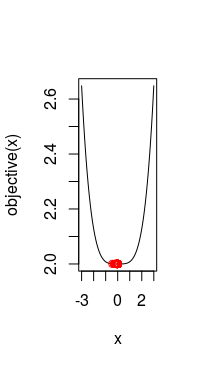
\includegraphics[scale=0.6]{../LDA/gradient_descent.png}
\end{column}
\end{columns}

}
\end{document}

